\chapter{Medical Imaging and Image Segmentation}
%

%%%%%%%%%%%%%%%%%%%%%%%%%%%%%%%%%%%%%%%%%%%%%%%
%%%%%%%%%%%%%%%%%%%%%%%%%%%%%%%%%%%%%%%%%%%%%%%
\section{Review of Imaging Techniques}
\label{Review of Imaging Techniques}

\subsection{Magnetic Resonance Imaging}
\label{Magnetic Resonance Imaging}

\subsection{X-Ray Computed Tomography}
\label{X-Ray Computed Tomography}

\subsection{Other Imaging Modalities}
\label{Other Imaging Modalities}

%%%%%%%%%%%%%%%%%%%%%%%%%%%%%%%%%%%%%%%%%%%%%%%
%%%%%%%%%%%%%%%%%%%%%%%%%%%%%%%%%%%%%%%%%%%%%%%
\section{Review of Image Segmentation Techniques}
\label{Review of Image Segmentation Techniques}

\begin{figure}[ht]
\centering
\subfigure[]{%
		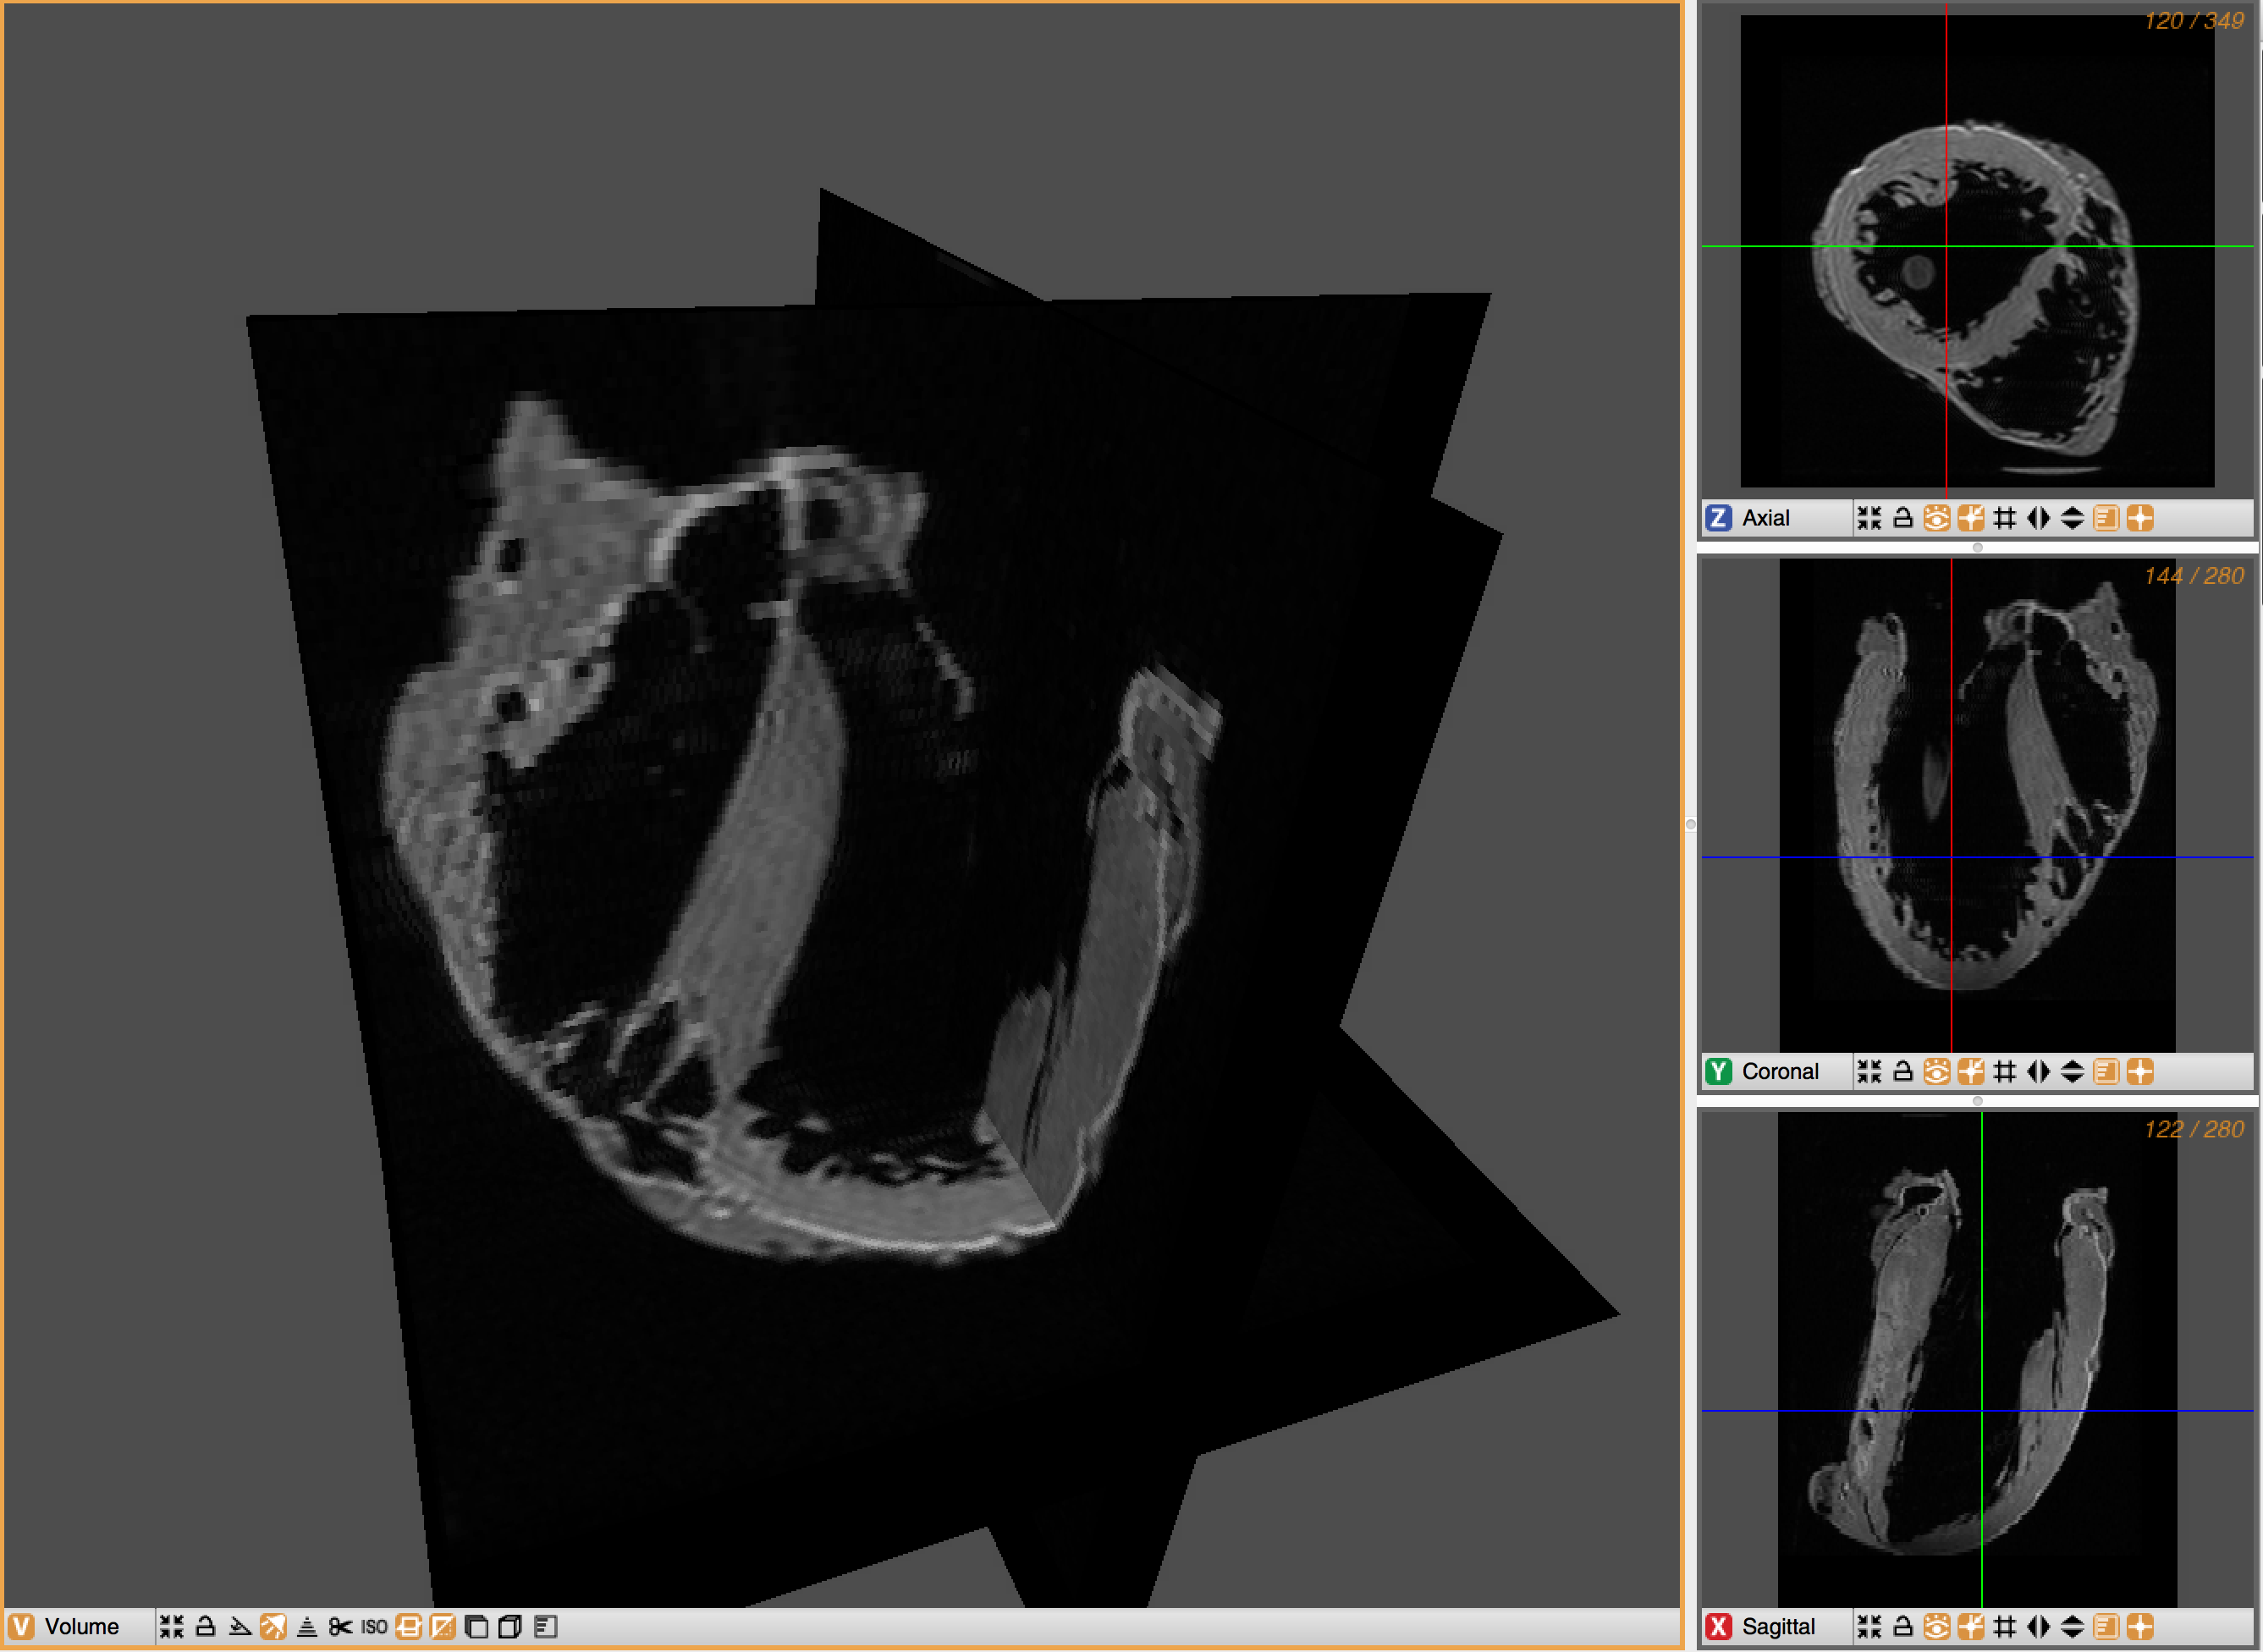
\includegraphics[scale=0.165]{media/1-seg3d/1-raw.png}
\label{fig:seg1}}
\subfigure[]{%
		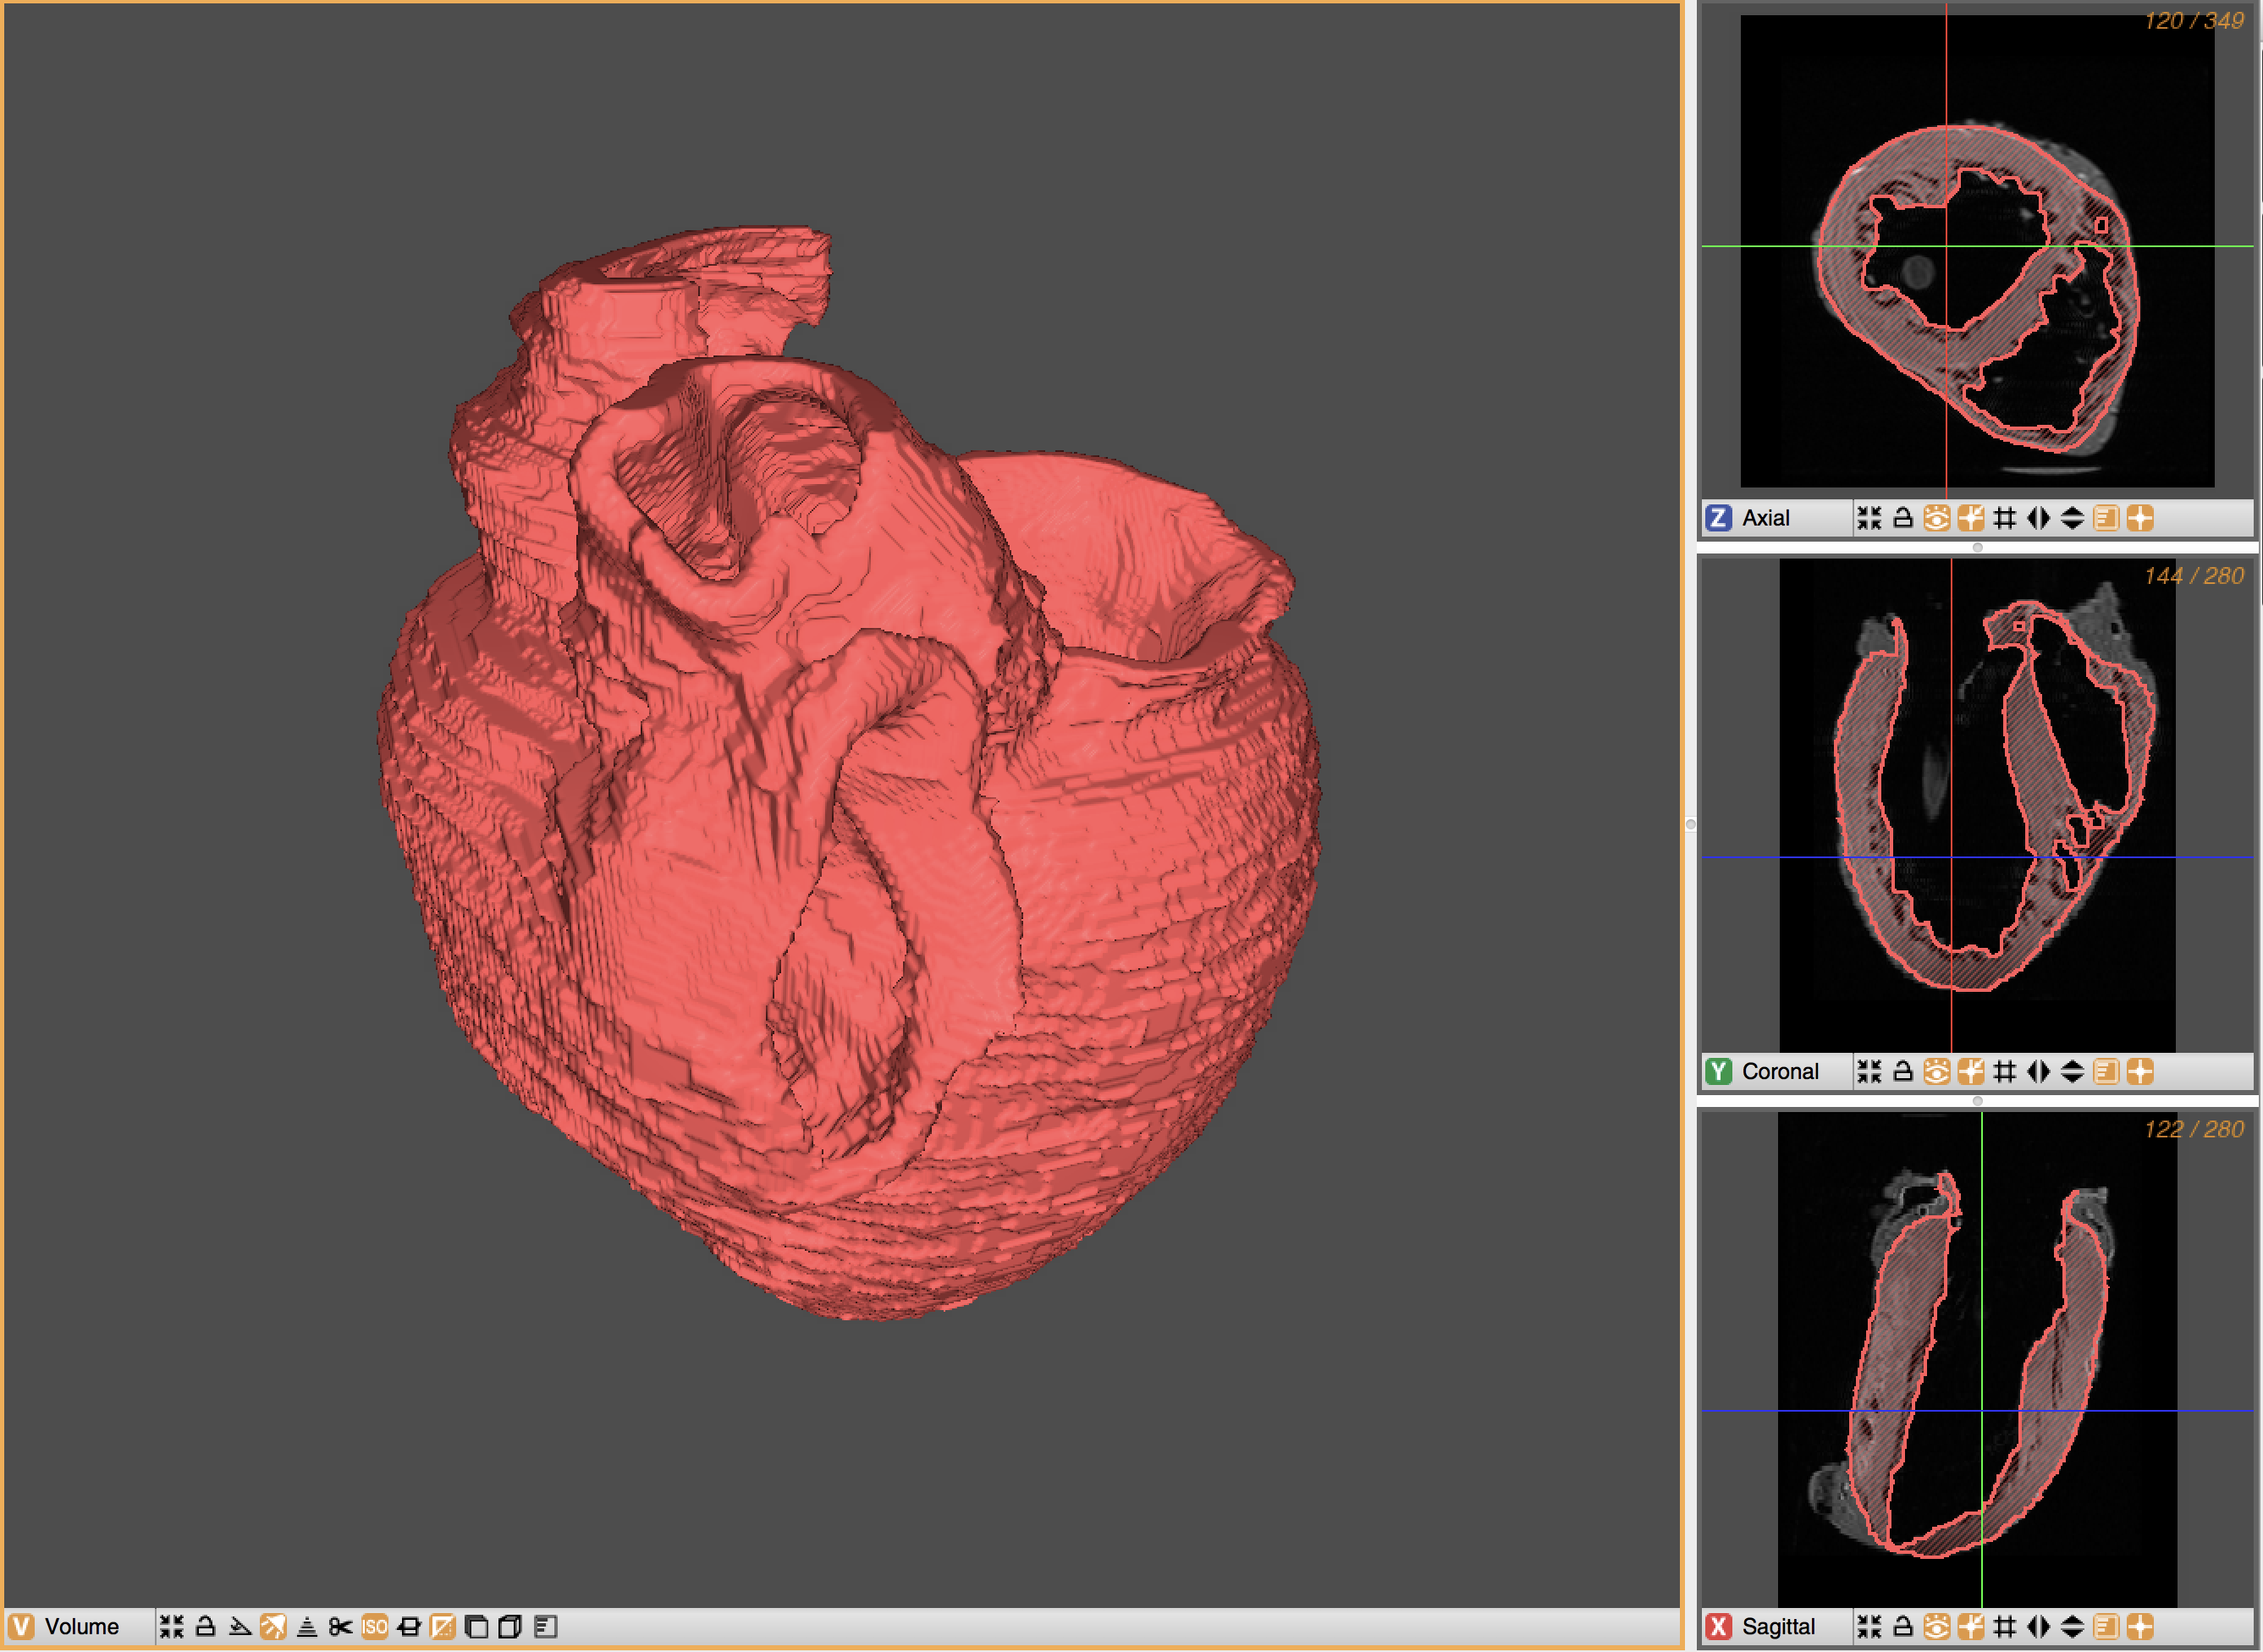
\includegraphics[scale=0.165]{media/1-seg3d/2-seg.png}
\label{fig:seg2}}
%
\caption{(a) MRI of \textit{ex-vivo} human heart, and (b) resulting segmented image mask}
\label{fig:seg}
\end{figure}